\chapter{Integration strategy}


\section{Entry criteria}
Before the integration testing phase proper may begin, it is important that the code has been inspected, manually or otherwise, and that unit tests have been run, so that any bug or issue found in this phase may be safely flagged as being a problem of integration and not something that works as it shouldn't at a lower level.


\section{Elements to be integrated}
As detailed in the \emph{Design Document}, the architecture is organized in several higher level components themselves divided in lower level modules. Refer to the \emph{Design Document} itself for a detailed listing of the elements.
\begin{figure}
\centering
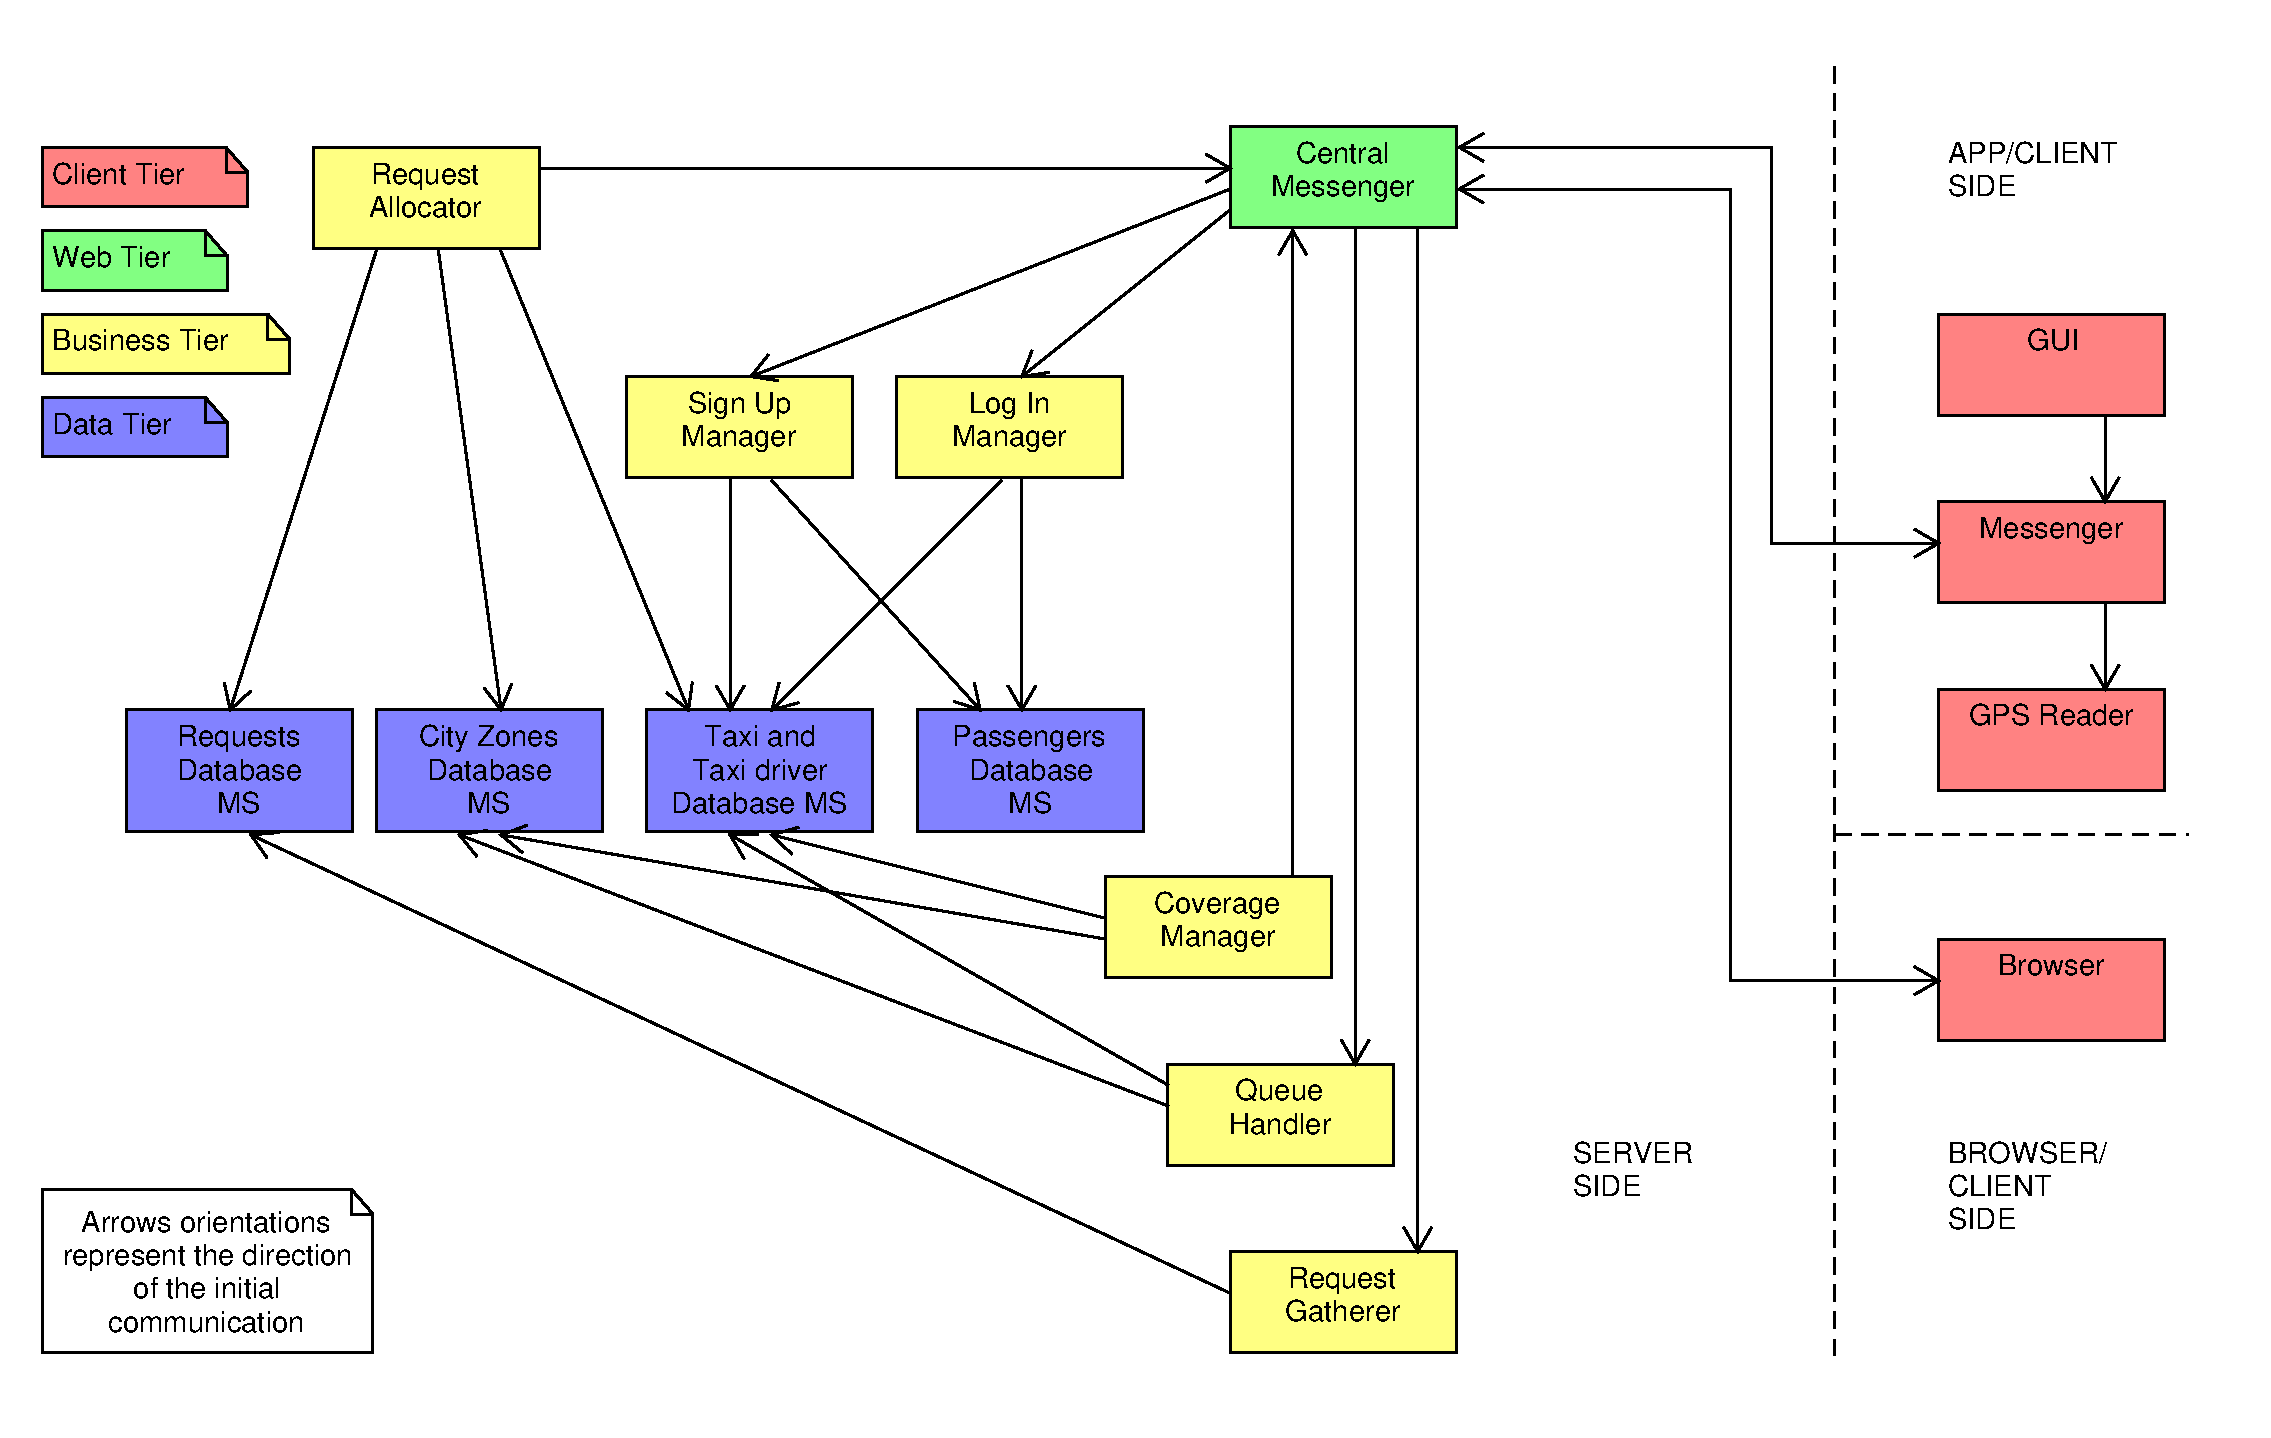
\includegraphics[width=\textwidth]{tex-images/interactions}
\caption{The different architectural components and their interaction -- see the \emph{Design Document}}
\end{figure}


\section{Integration testing strategy}
Since, as stated, the high level components are divided in low level modules, it is at first necessary to test the integration of the modules that make a single component before that same component can be tested against the others at the higher level.

A top down approach will be followed for the integration of the components. The process is very much simplified by the almost complete independence of most of the different components. As for the modules, since their number is rather small, a top down or functional grouping approach can be used indifferently without much impact overall.


\section{Sequence of integration}

\subsection{Components}
Since a top down (from the interface) approach will be used, the integration order will be as follow:
\begin{enumerate}
\item Client App GUI;
\item Client App Messenger;
\item Client App GPS Reader;
\item Client Webapp (on par with the three previous components);
\item Central messenger;
\item Log in manager;
\item Sign up magager;
\item Request allocator;
\item Coverage manager;
\item Queue handler;
\item Request gatherer;
\item All Database Management Systems.
\end{enumerate}

\subsection{Modules}